\section{Diagramas IDEF-0}\label{Ap:IDEF0}
\addcontentsline{toc}{section}{Apéndice 3: Diagramas IDEF-0} 
Estos son los diagramas IDEF0 que se han generado al momento de diseñar el sistema de compostaje.

\begin{figure}[h]
            \centering
            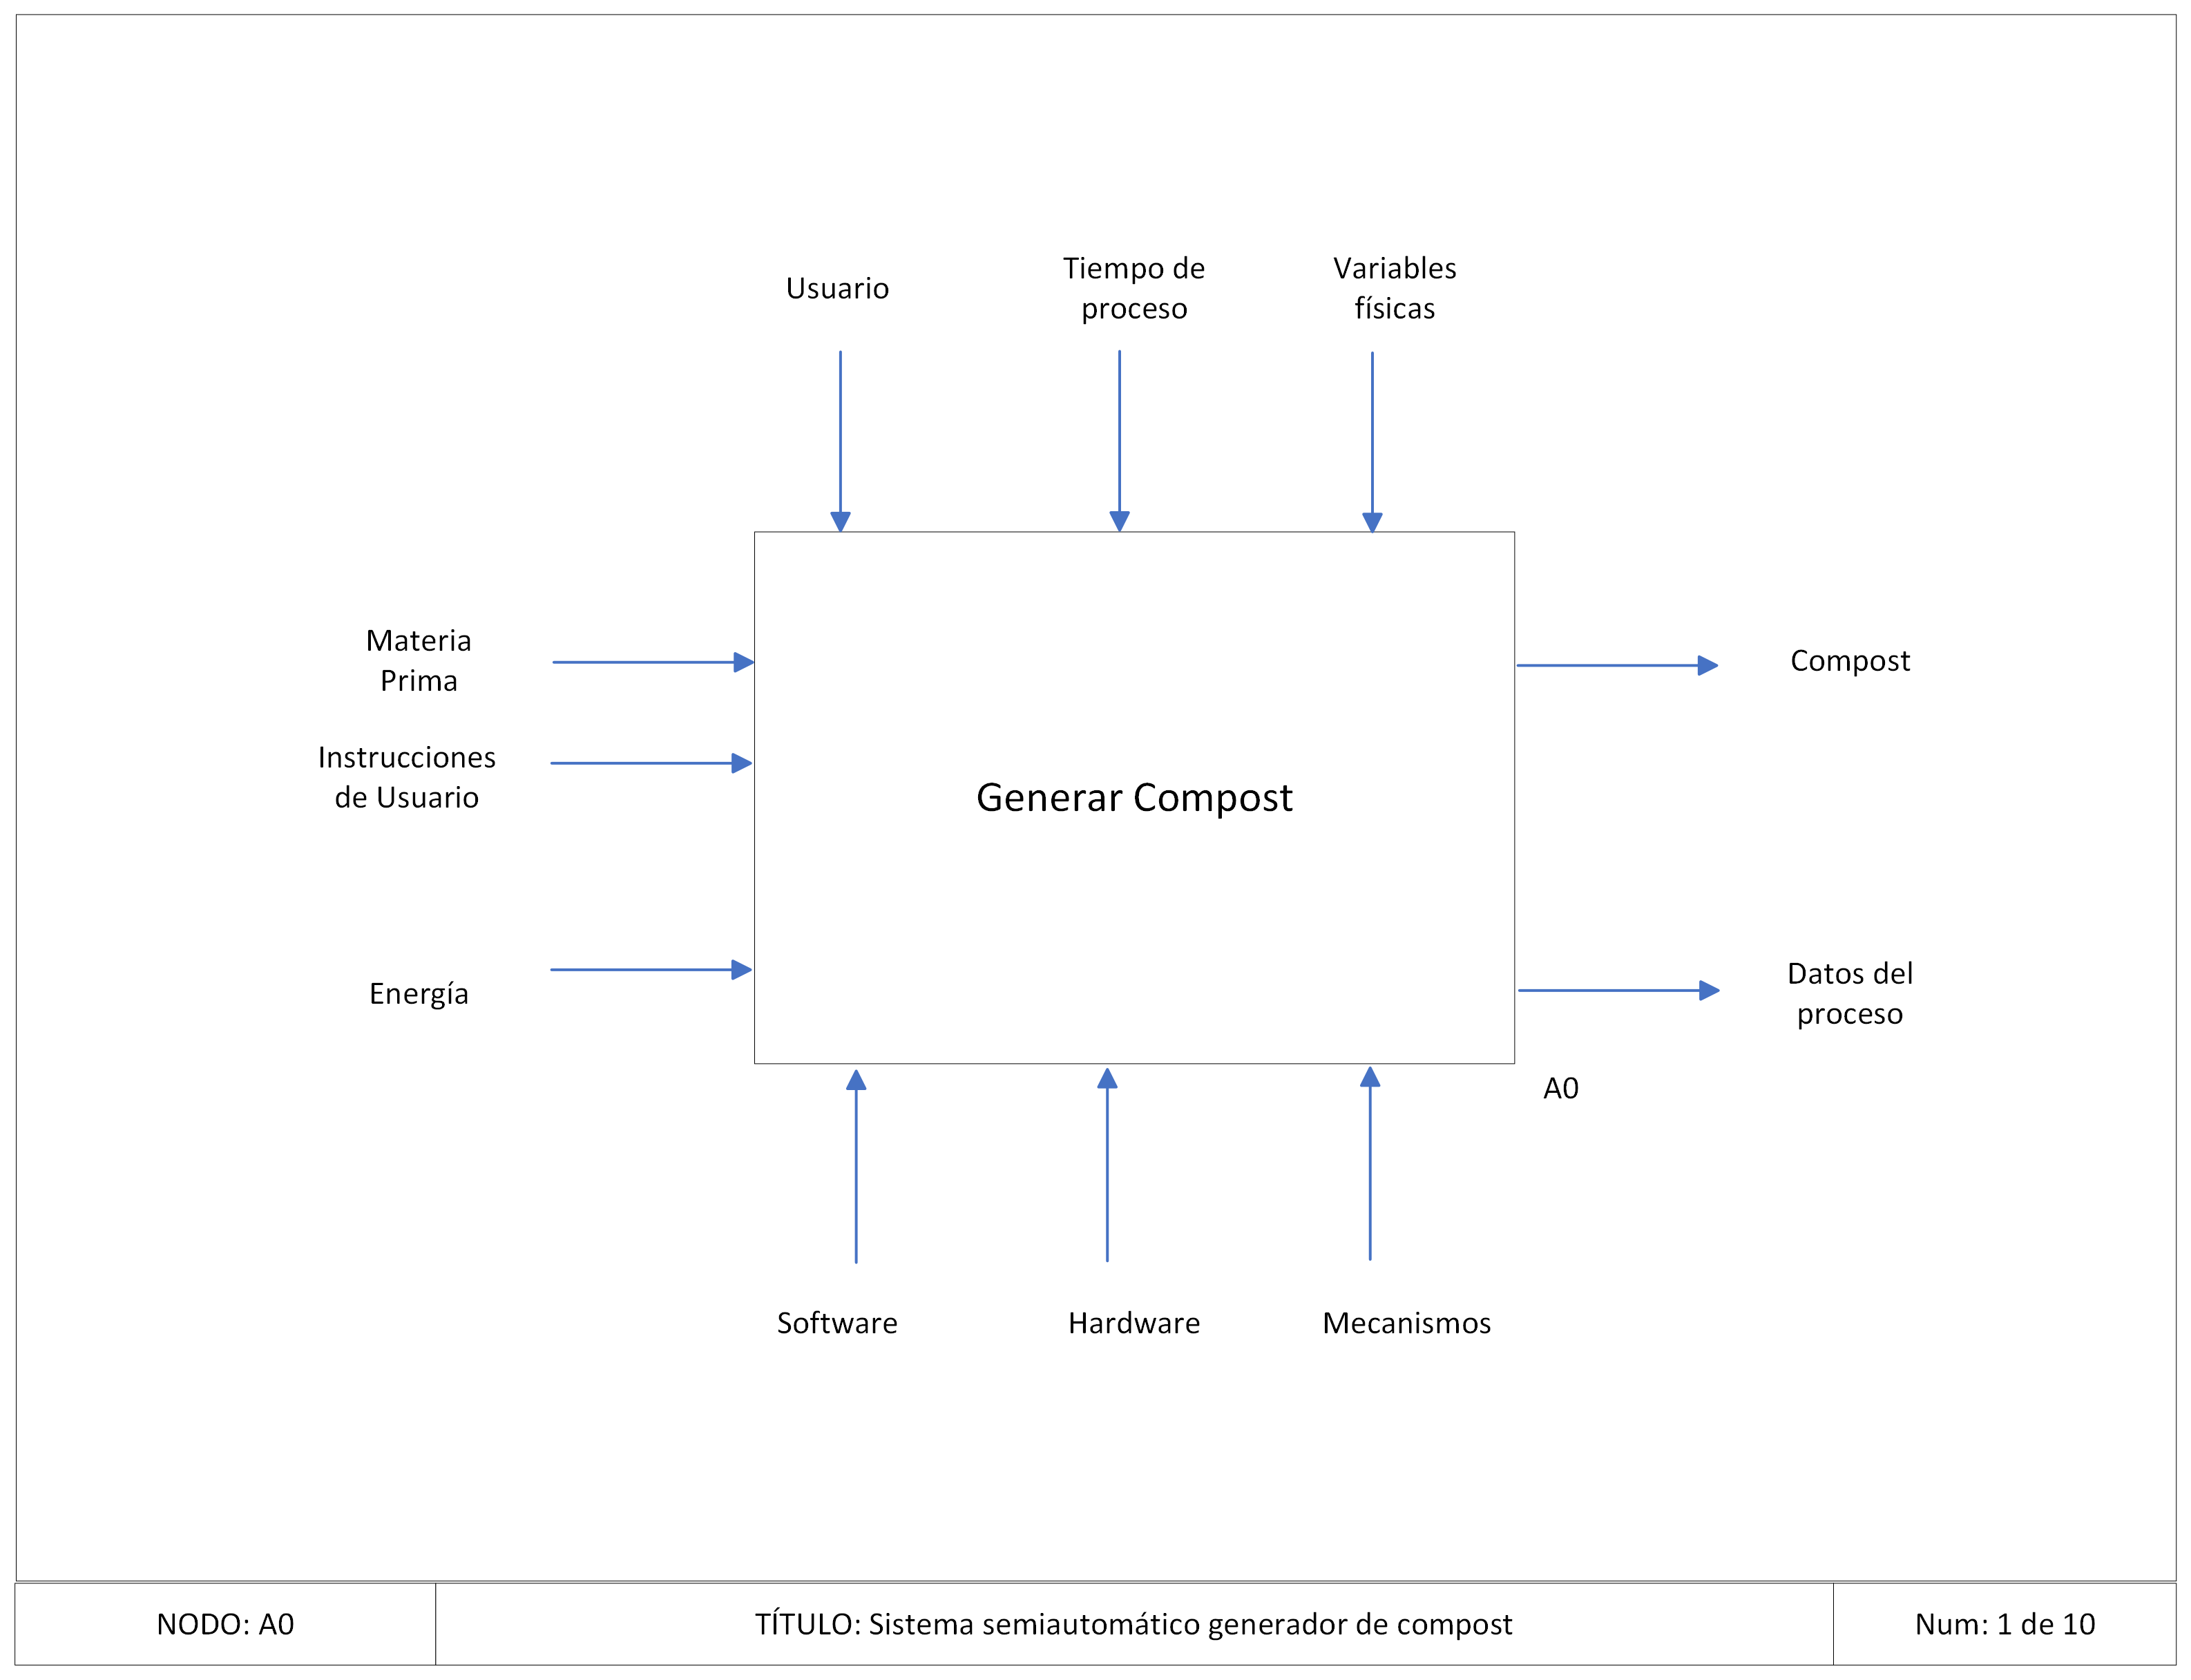
\includegraphics[scale=0.35, angle = 90]{images/Capitulo 6 Apéndices/01 IDEF 0/A0_final.png}
        \end{figure}
\newpage

\begin{figure}[h]
            \centering
            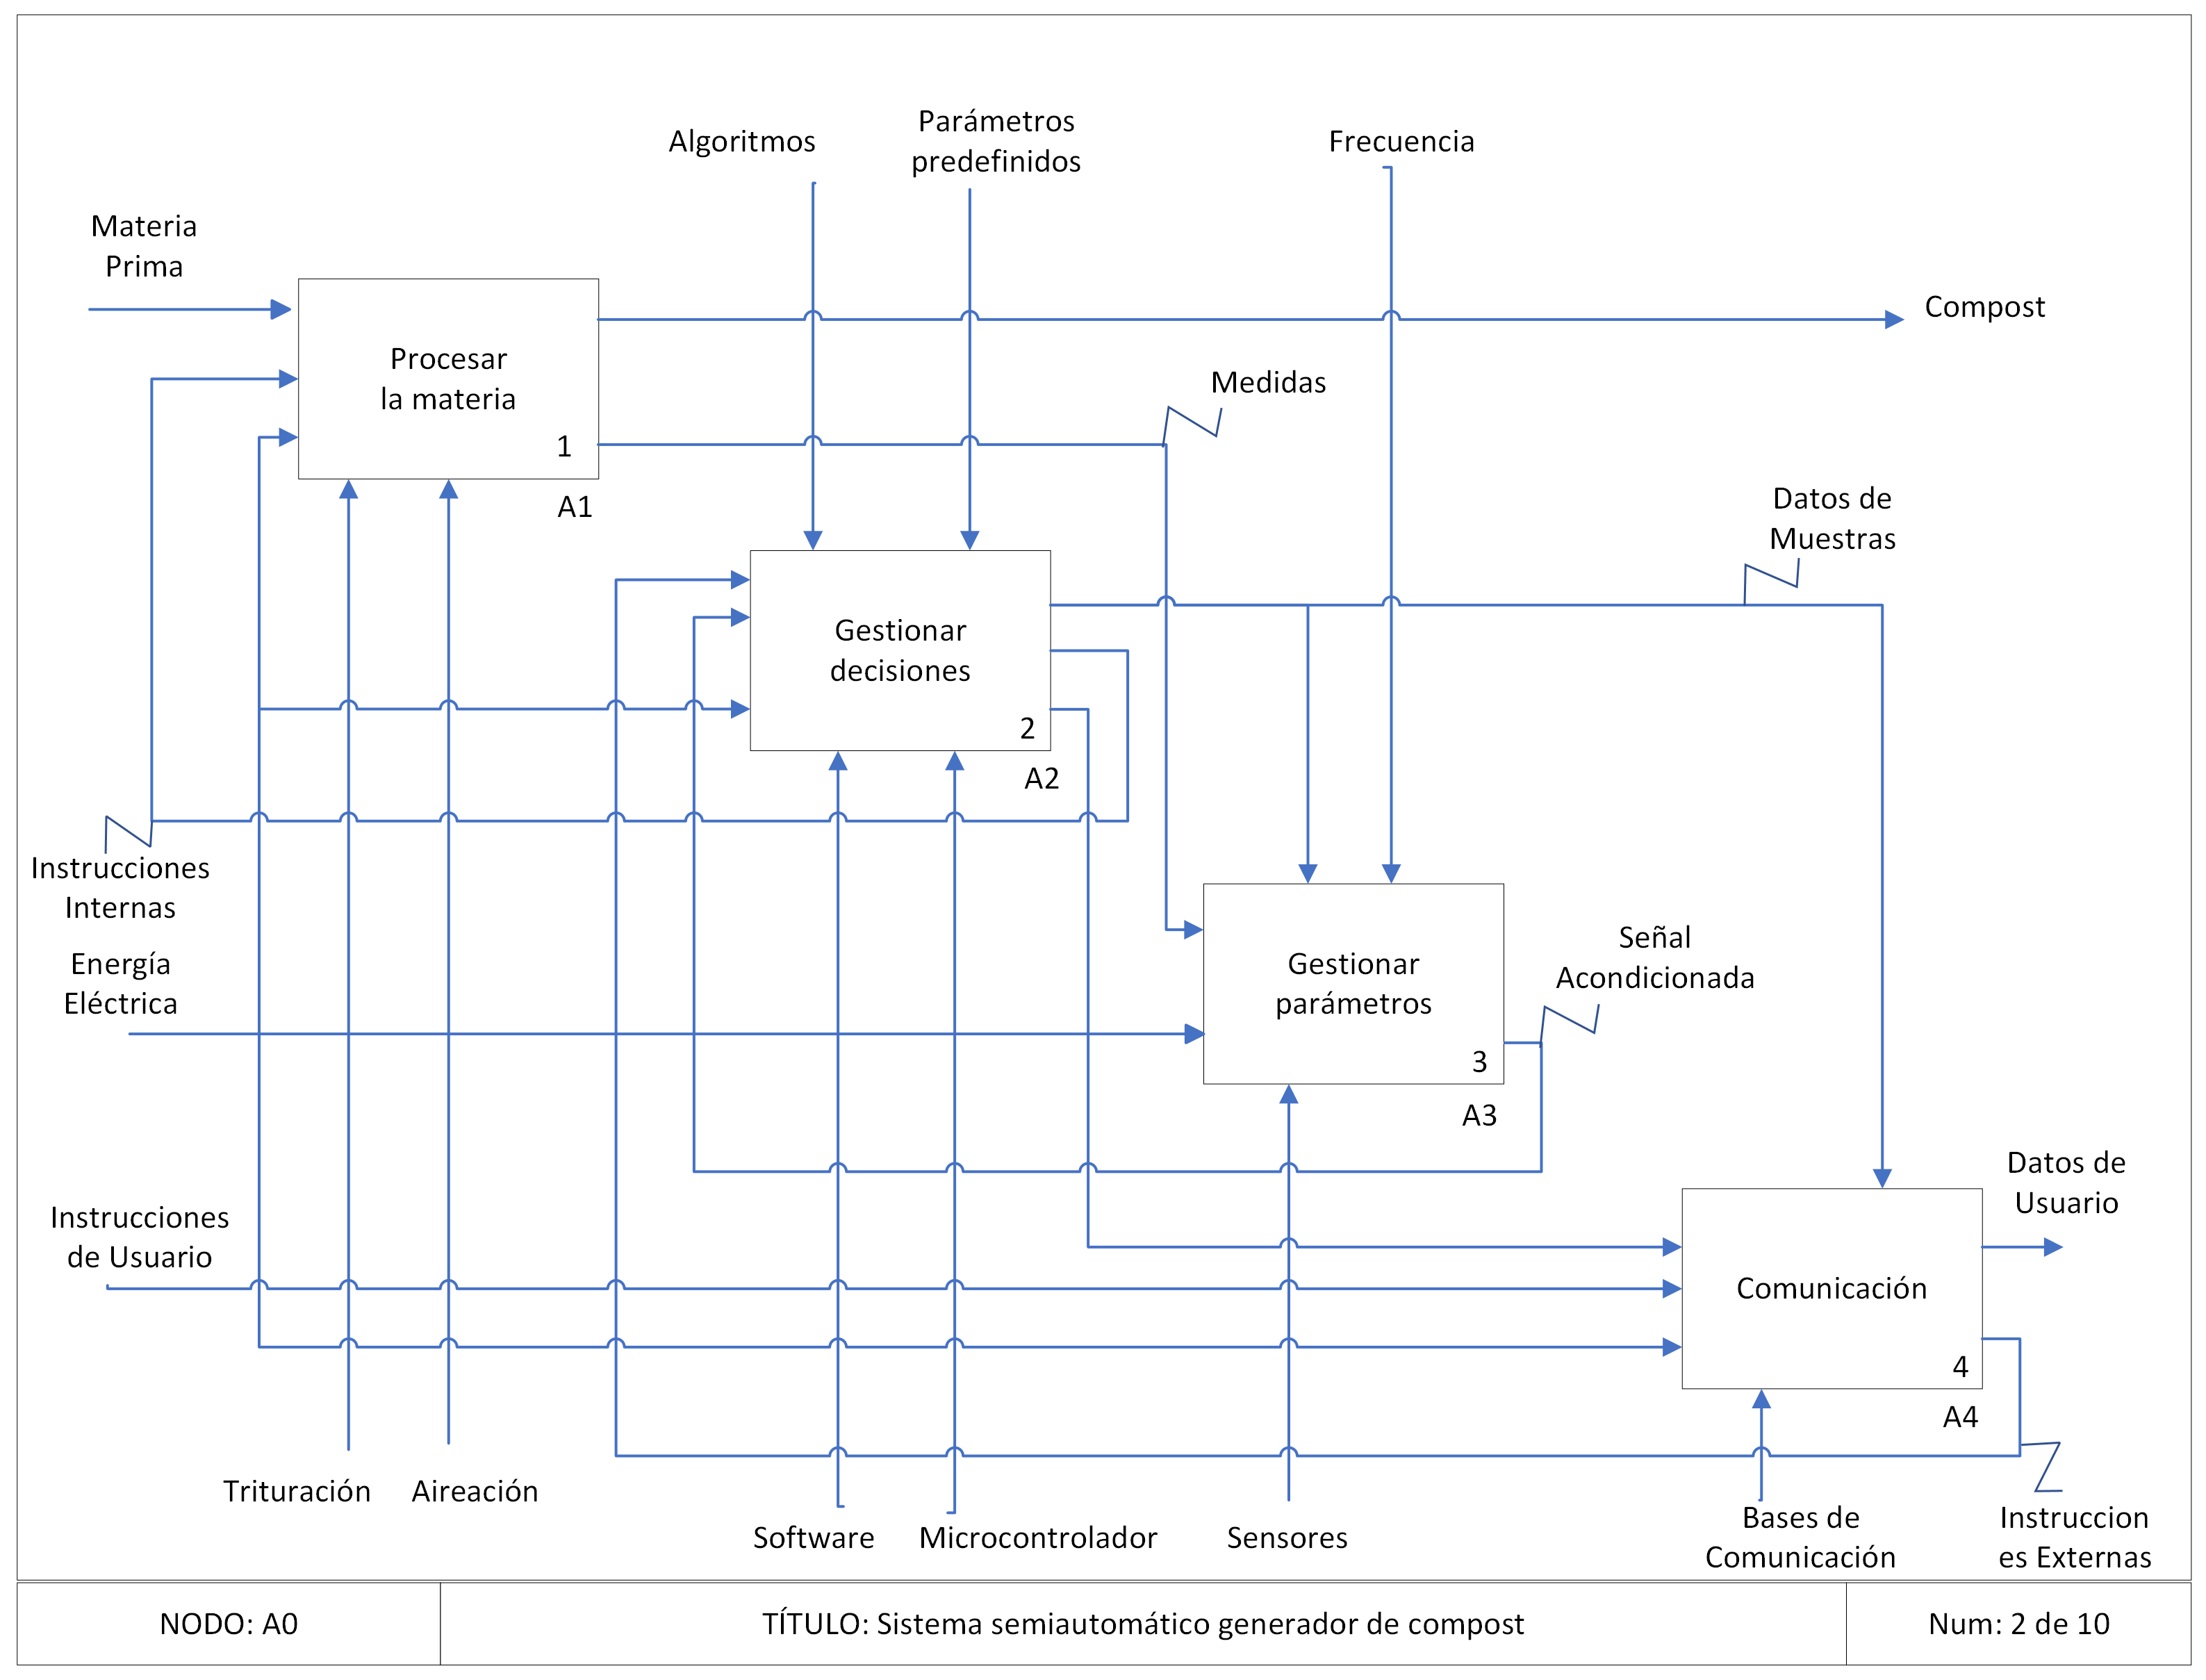
\includegraphics[scale=0.35, angle = 90]{images/Capitulo 6 Apéndices/01 IDEF 0/NodoA0.png}
        \end{figure}
\newpage

\begin{figure}[h]
            \centering
            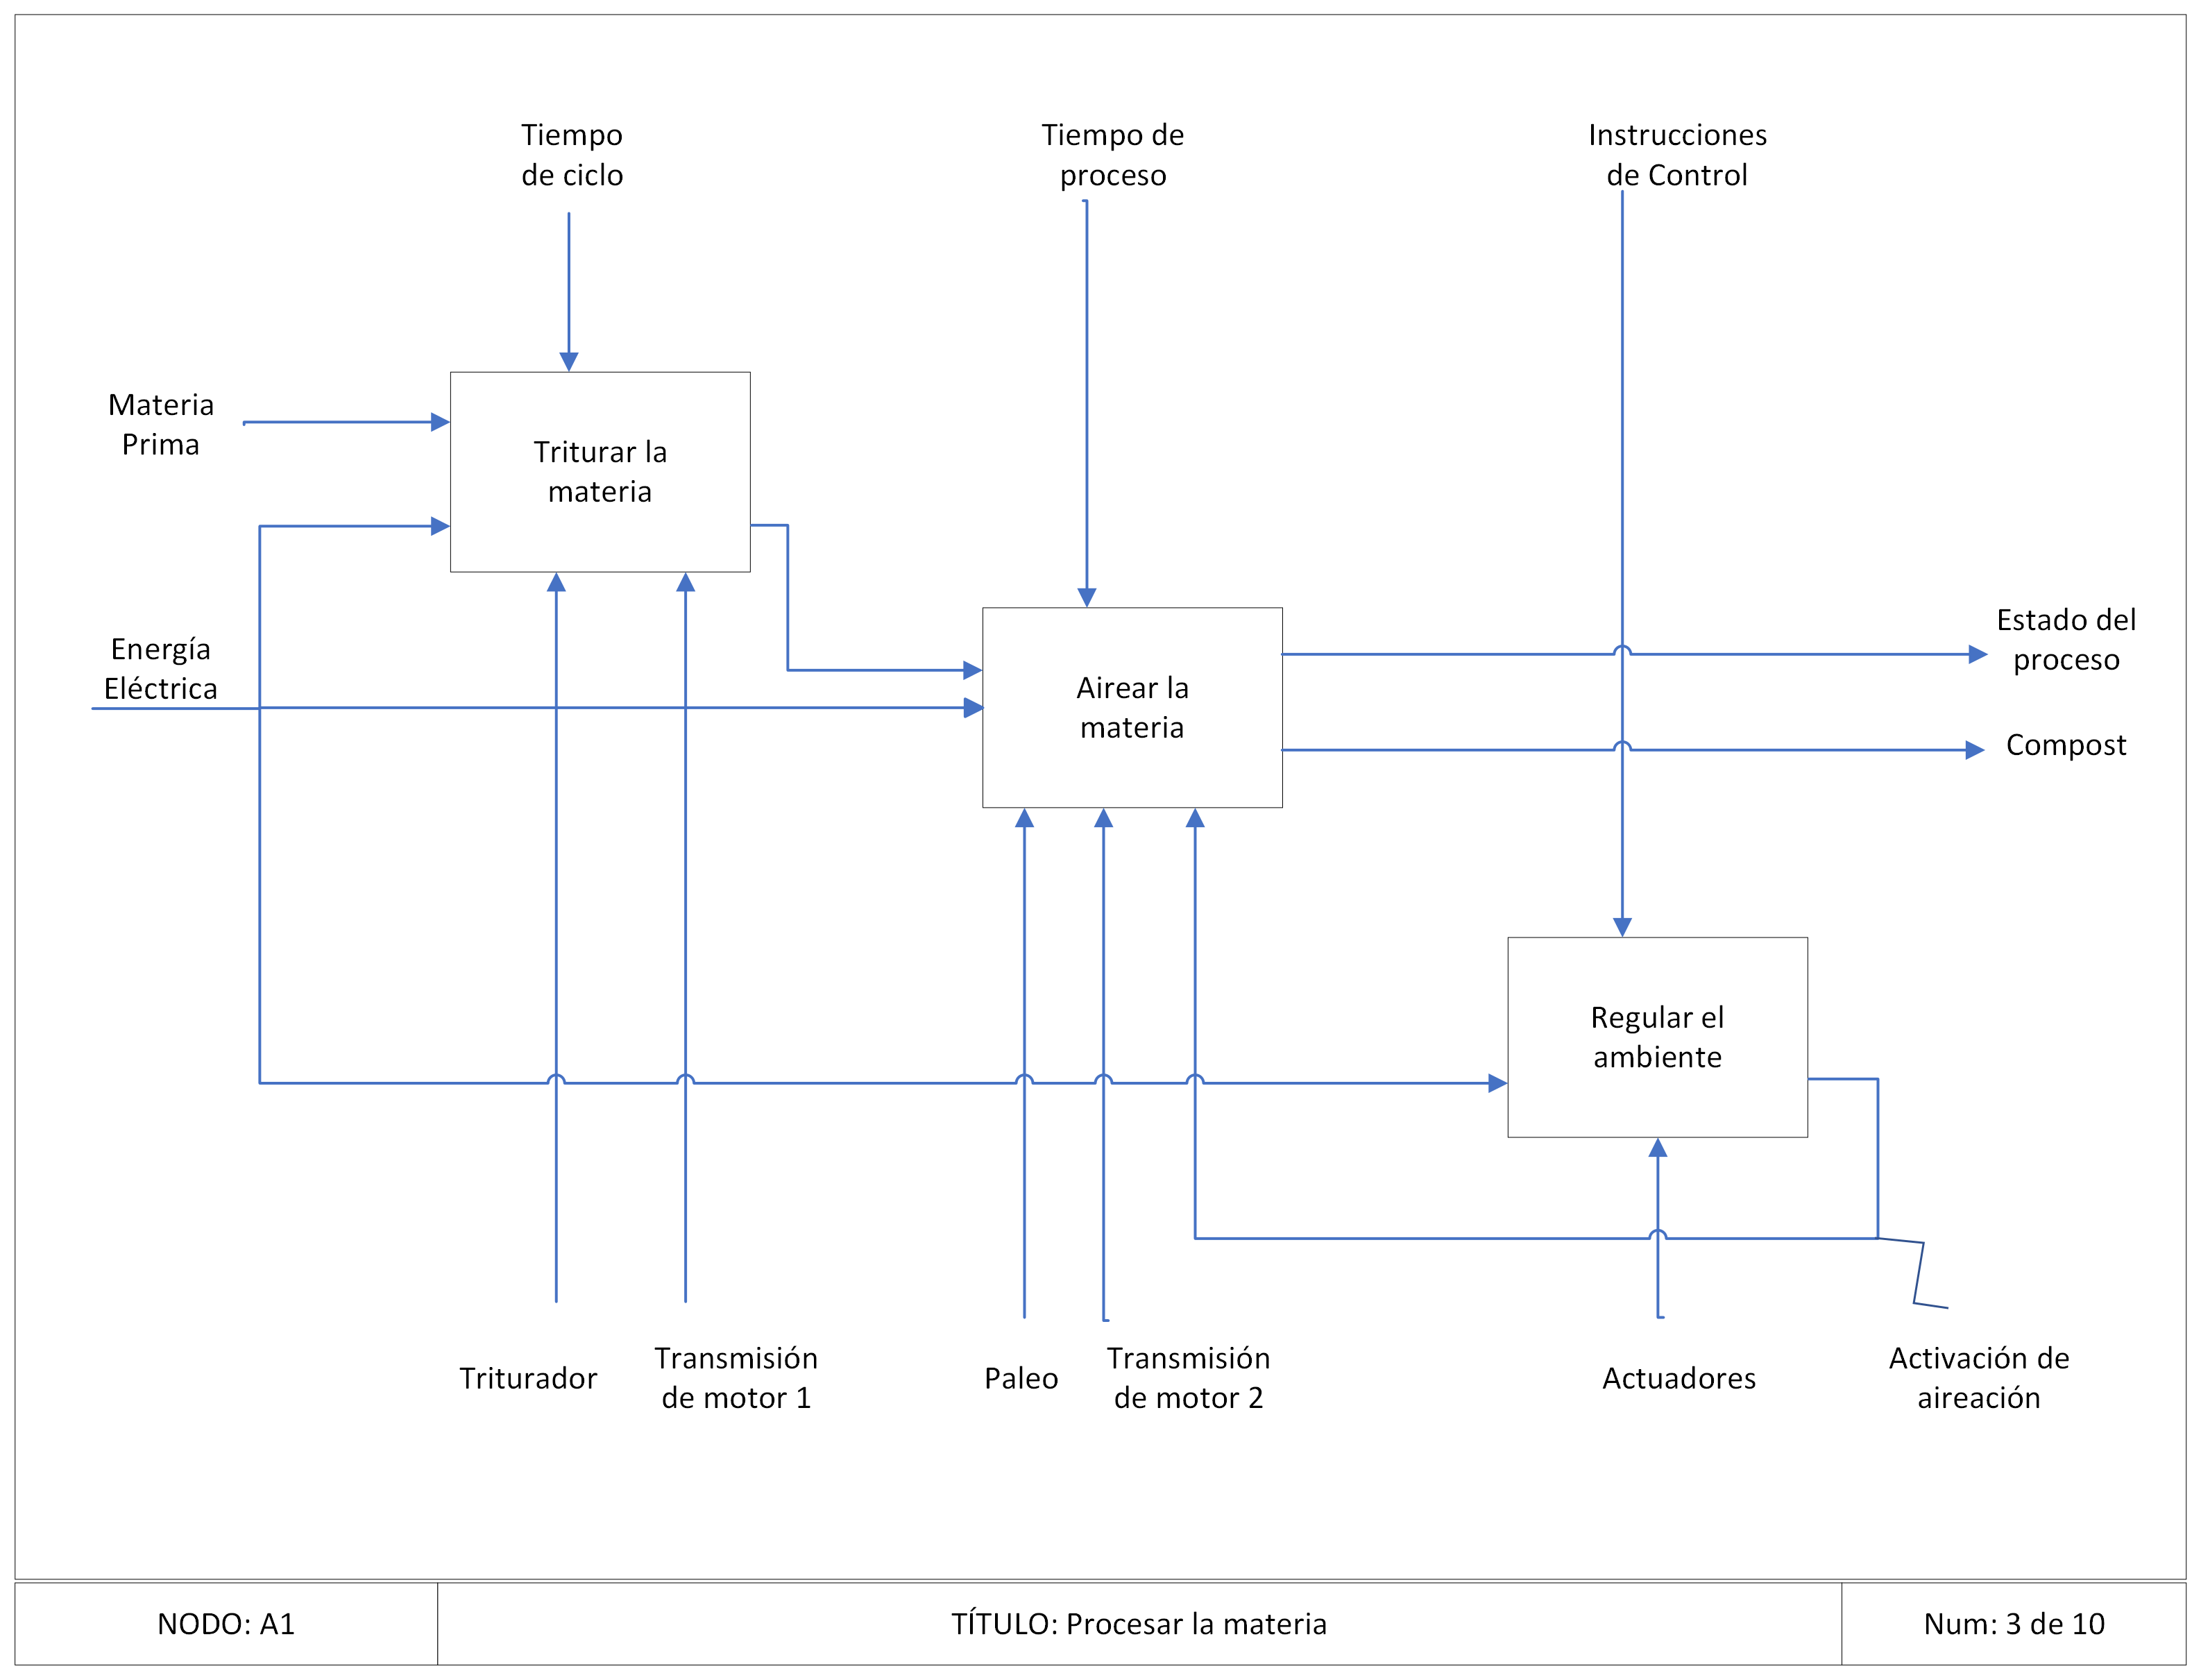
\includegraphics[scale=0.35, angle = 90]{images/Capitulo 6 Apéndices/01 IDEF 0/A1_final - Copy.png}
        \end{figure}
\newpage

\begin{figure}[h]
            \centering
            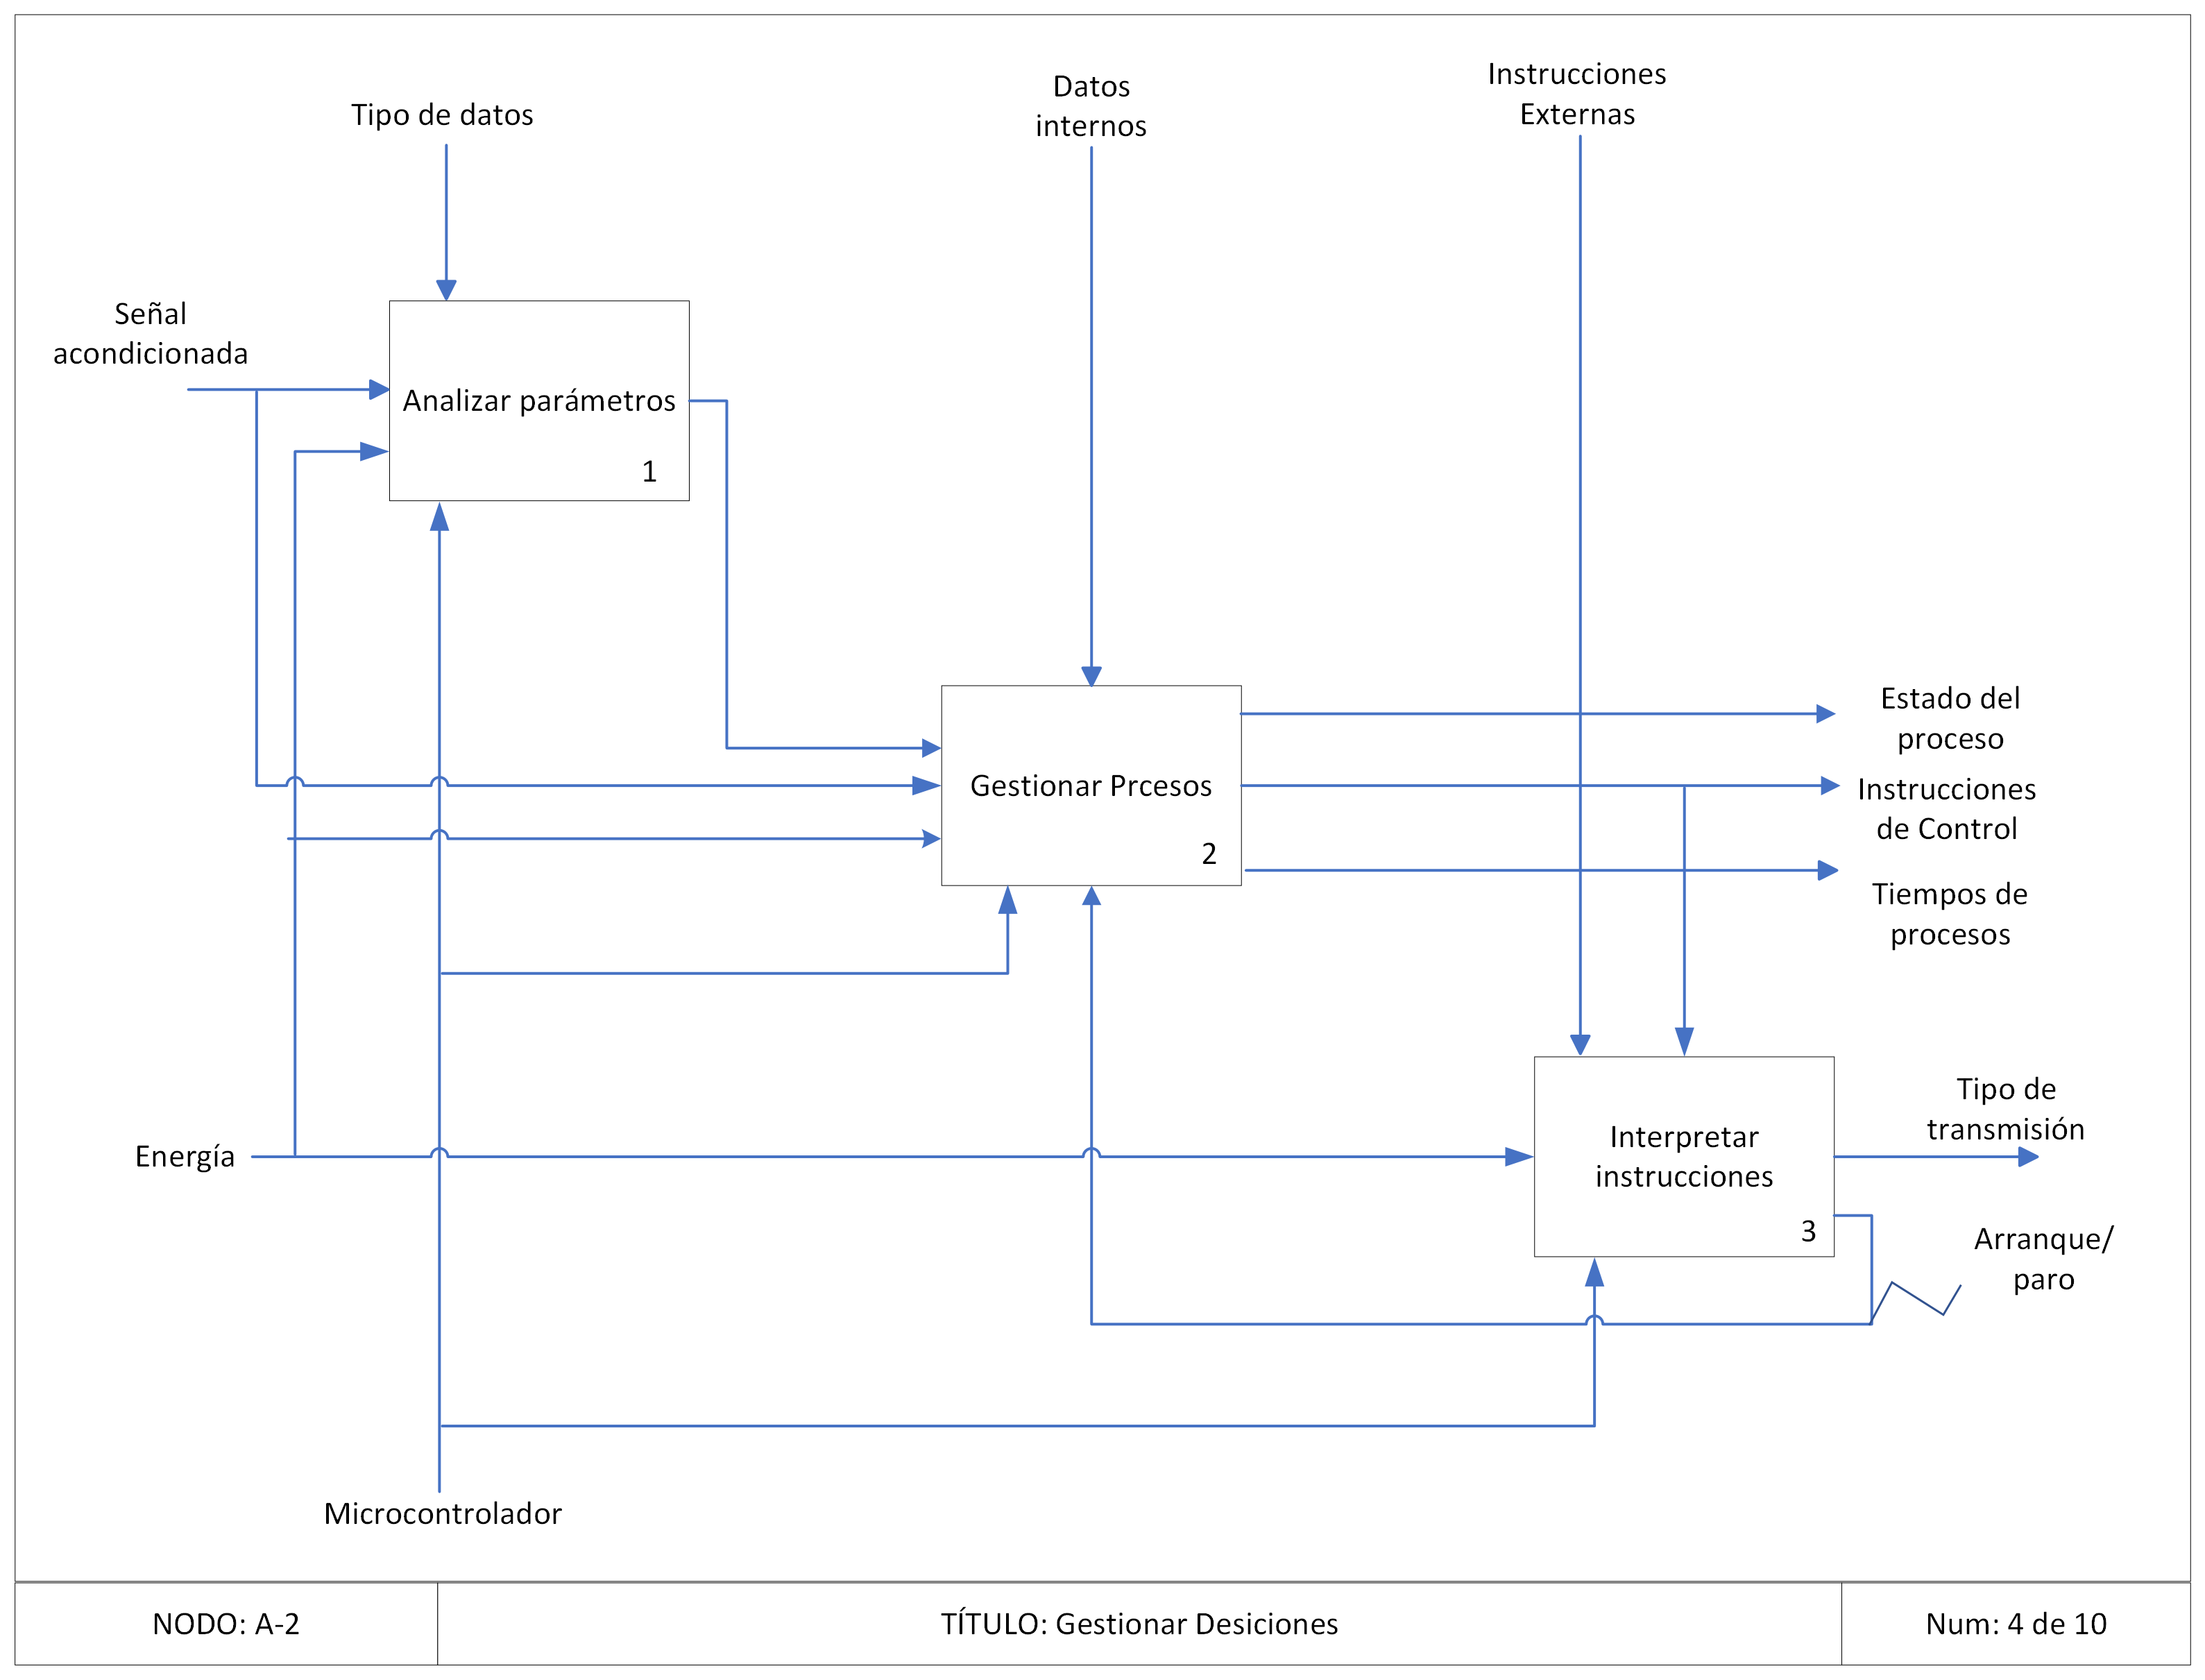
\includegraphics[scale=0.35, angle = 90]{images/Capitulo 6 Apéndices/01 IDEF 0/A2_conmarco - Copy.png}
        \end{figure}
\newpage

\begin{figure}[h]
            \centering
            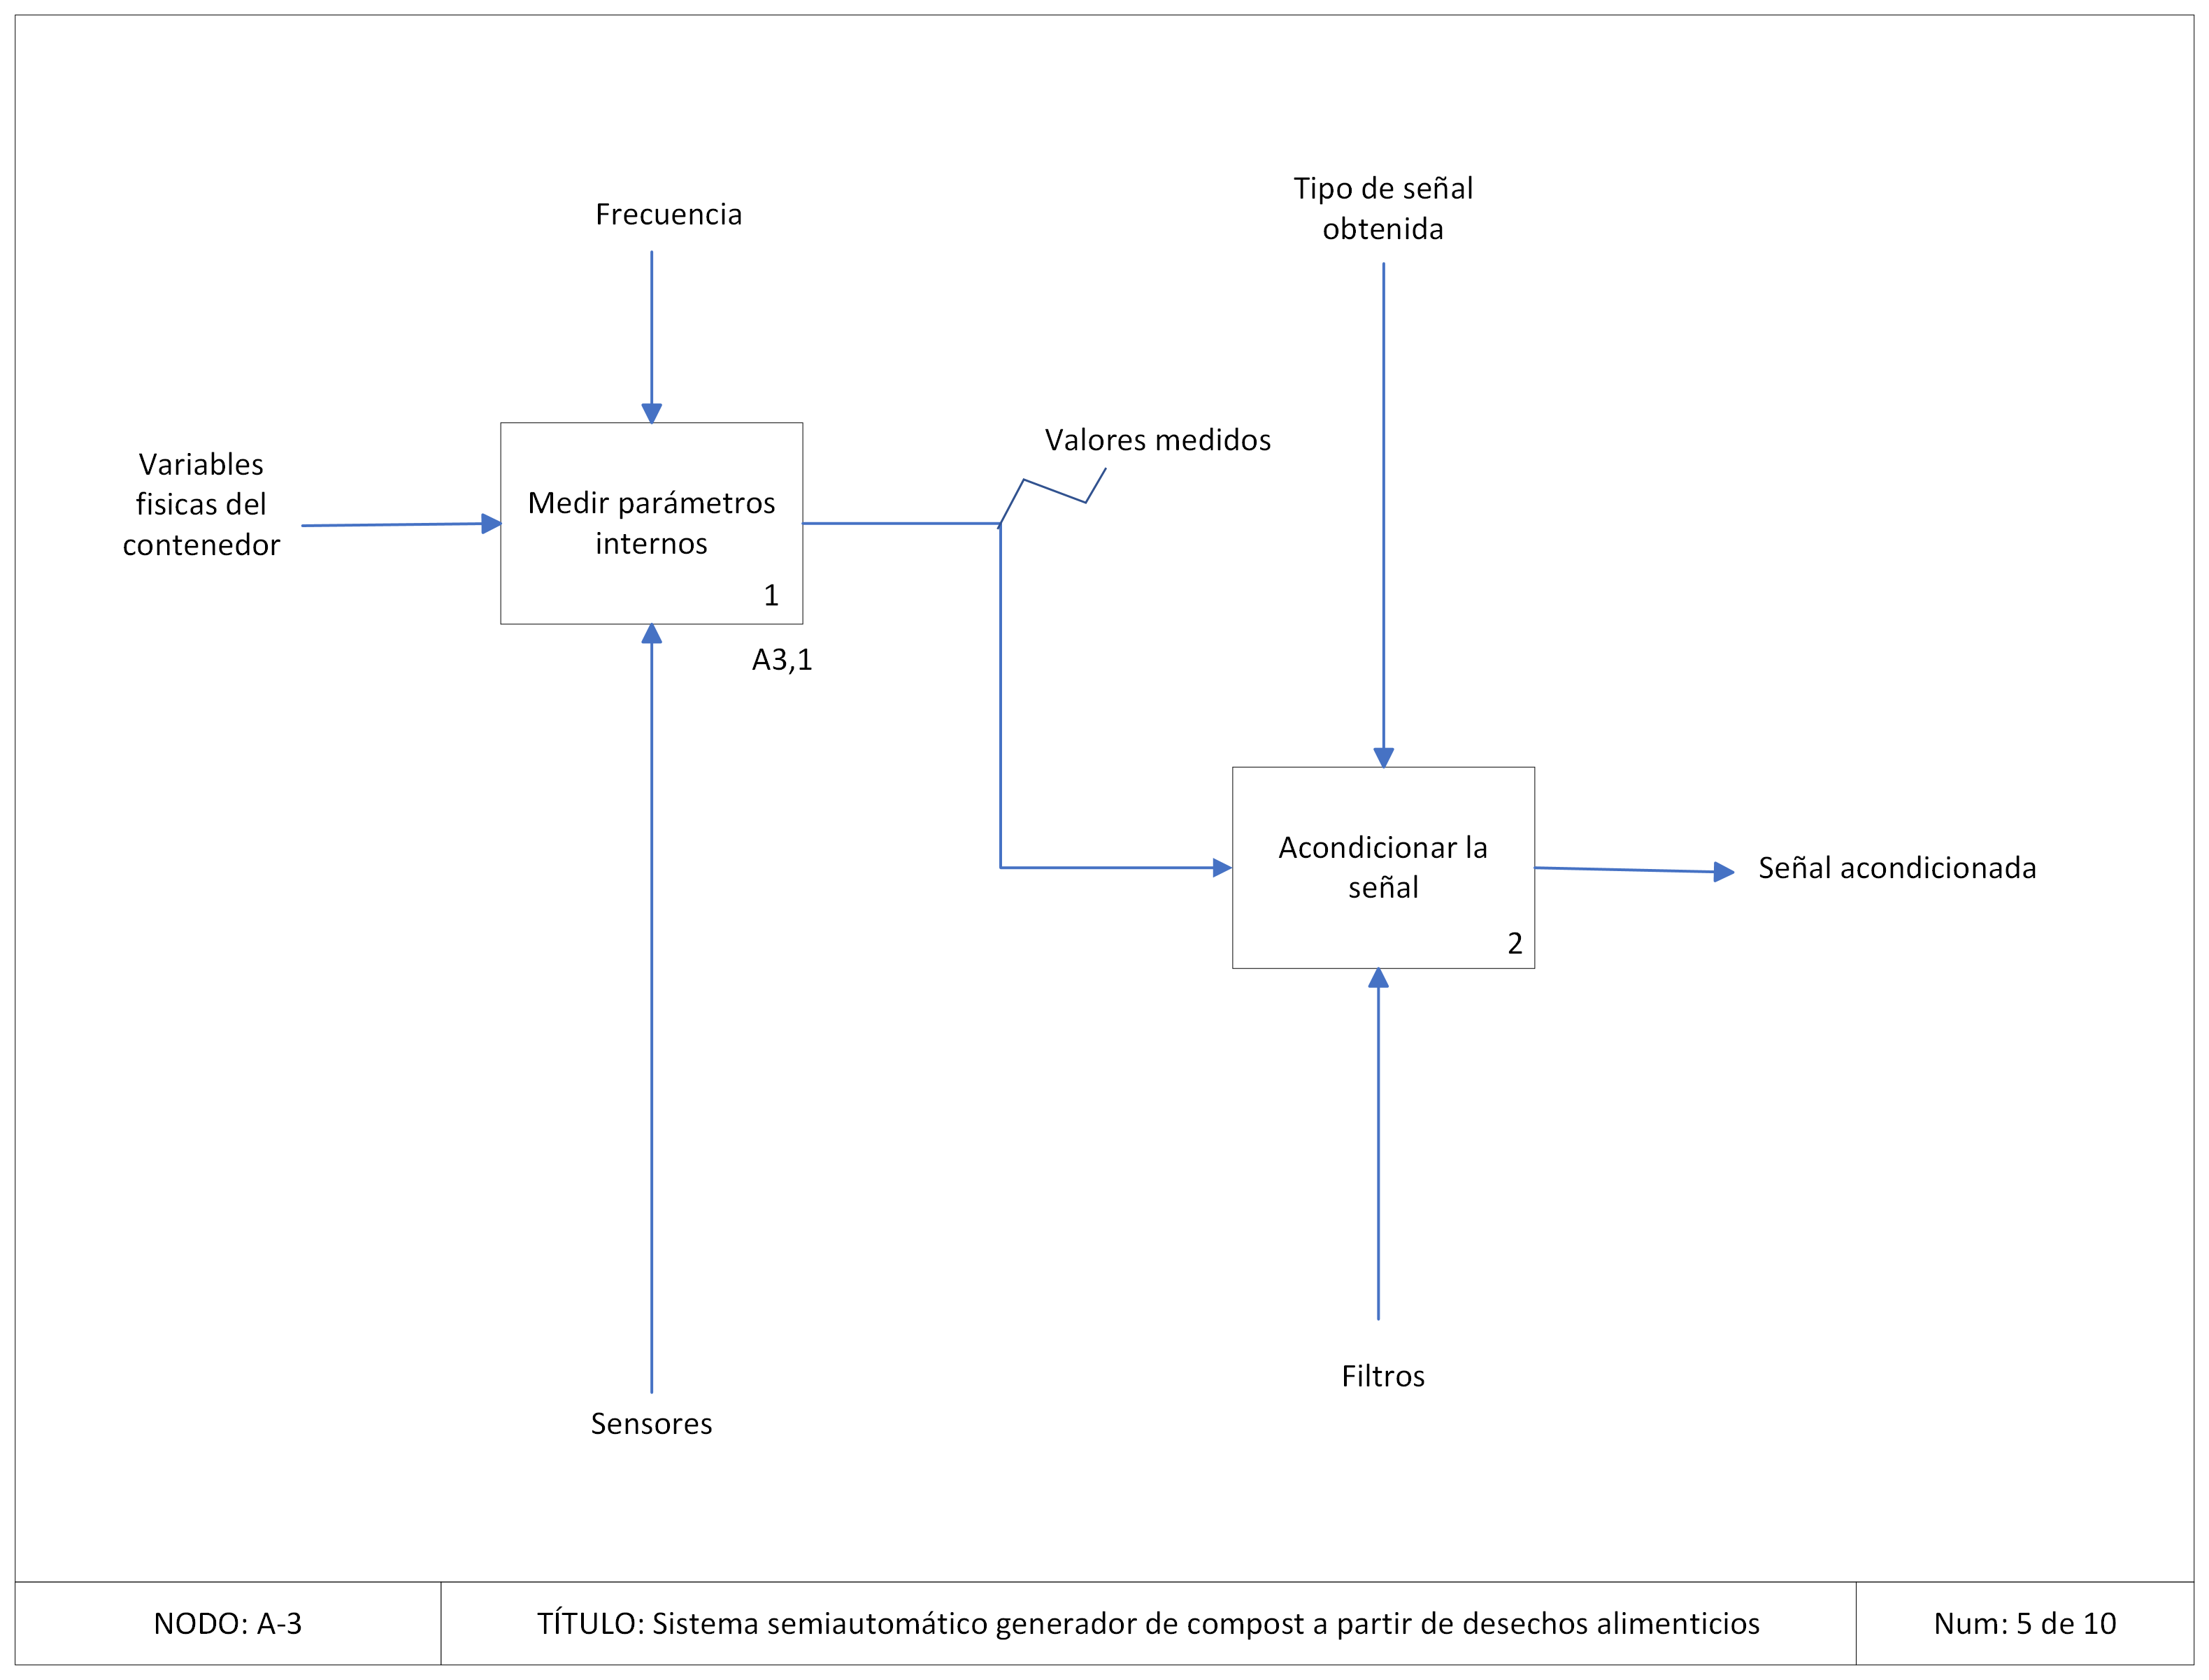
\includegraphics[scale=0.35, angle = 90]{images/Capitulo 6 Apéndices/01 IDEF 0/A3_conmarco - Copy.png}
        \end{figure}
\newpage

\begin{figure}[h]
            \centering
            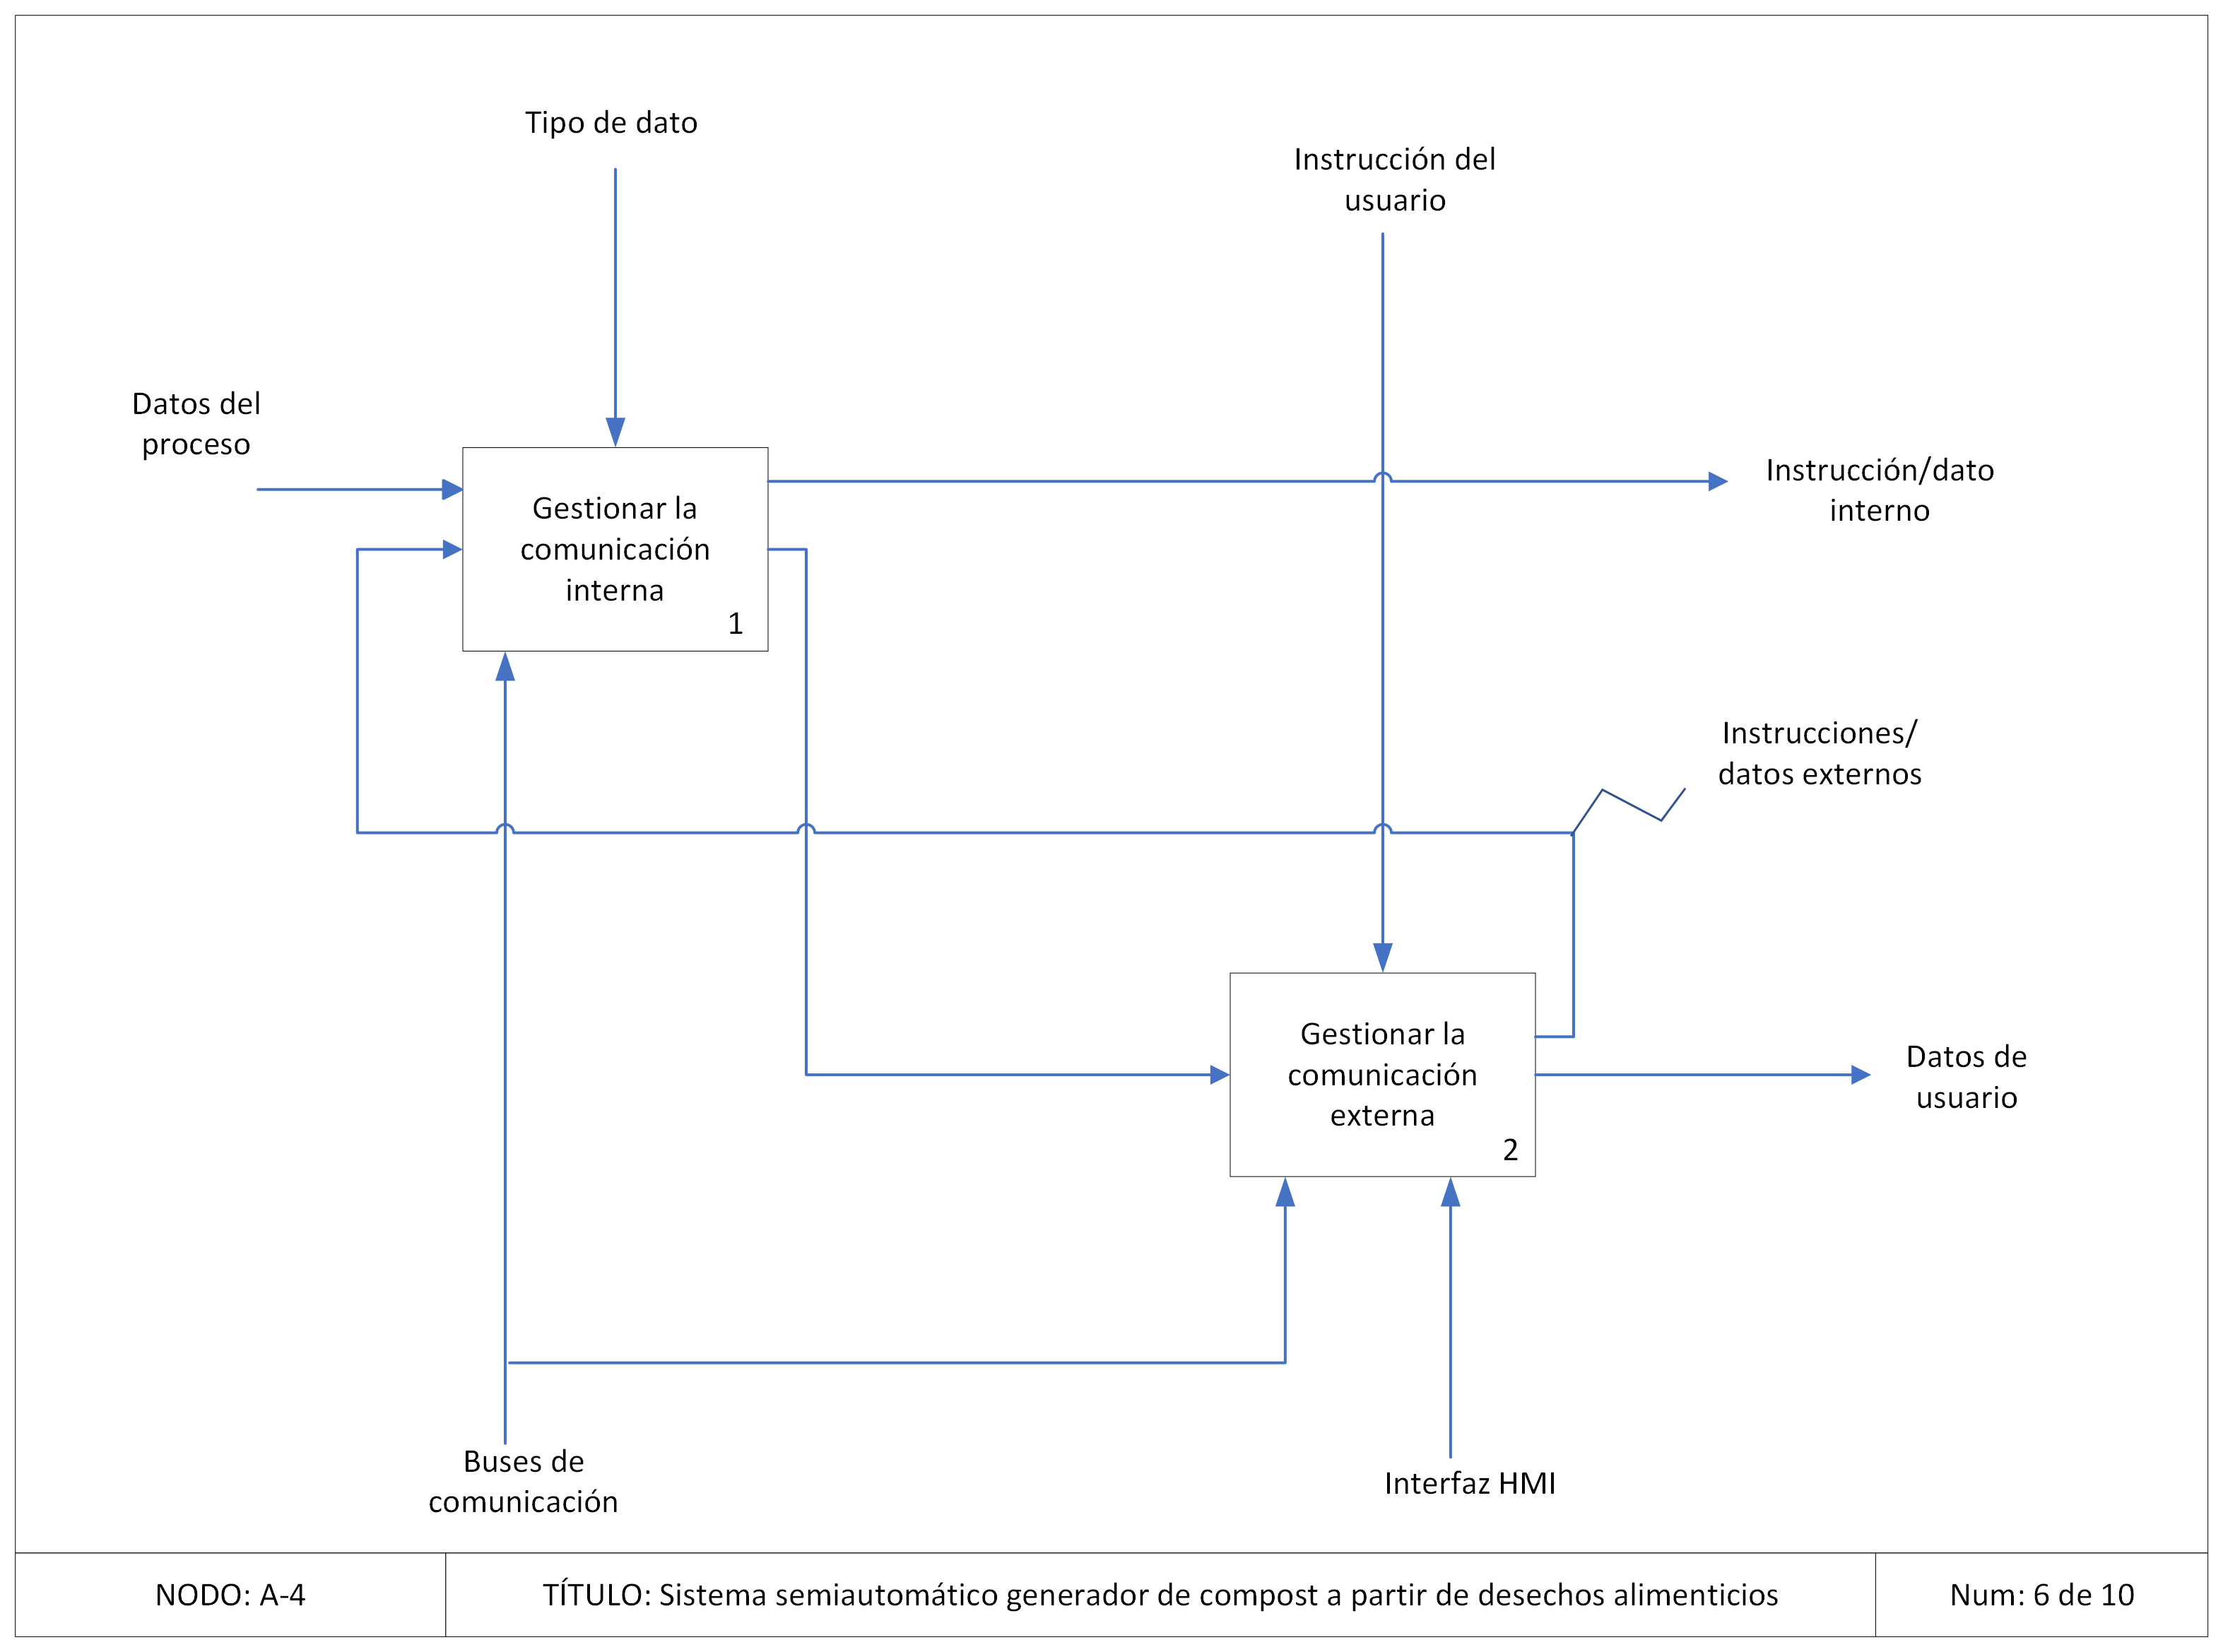
\includegraphics[scale=0.35, angle = 90]{images/Capitulo 6 Apéndices/01 IDEF 0/A4_conmarco - Copy.png}
        \end{figure}
\newpage

%\begin{figure}[h]
%            \centering
%            \includegraphics[scale=0.35, angle = 90]{images/Capitulo 6 Apéndices/01 IDEF 0/A5_conmarco - Copy.png}
%        \end{figure}
%\newpage

\begin{figure}[h]
            \centering
            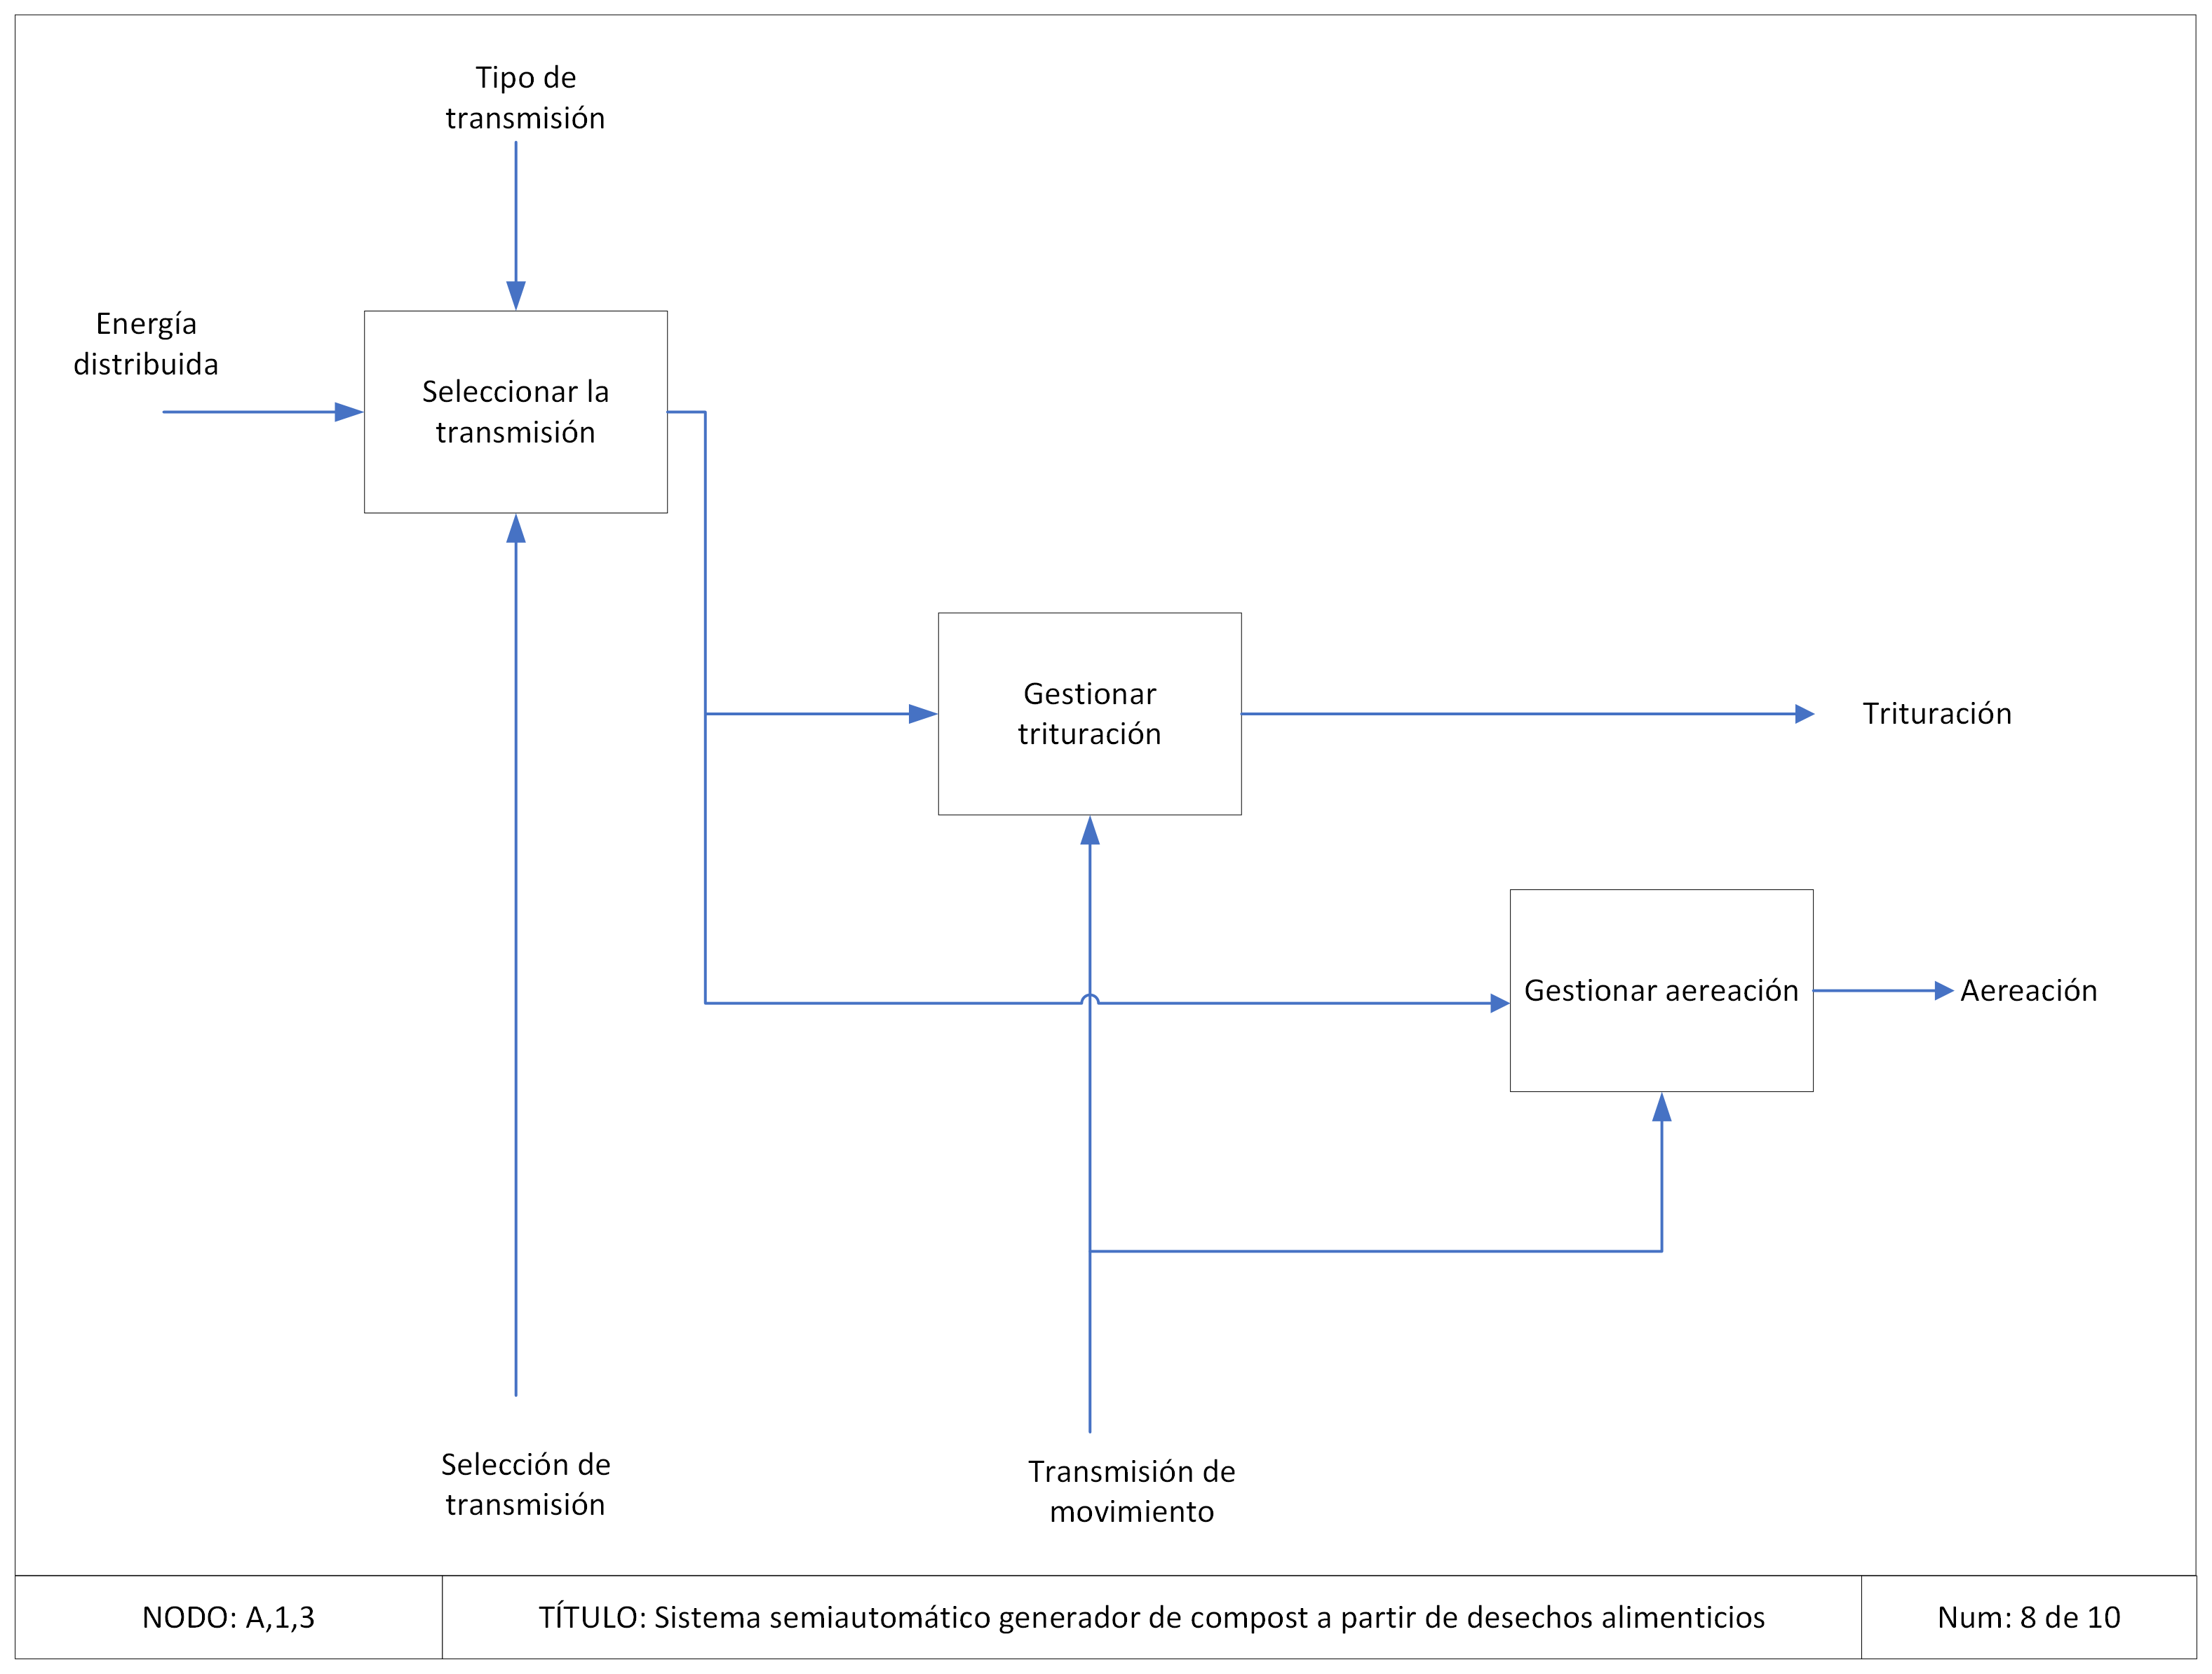
\includegraphics[scale=0.35, angle = 90]{images/Capitulo 6 Apéndices/01 IDEF 0/A,1,3_conmarco - Copy.png}
        \end{figure}
\newpage

\begin{figure}[h]
            \centering
            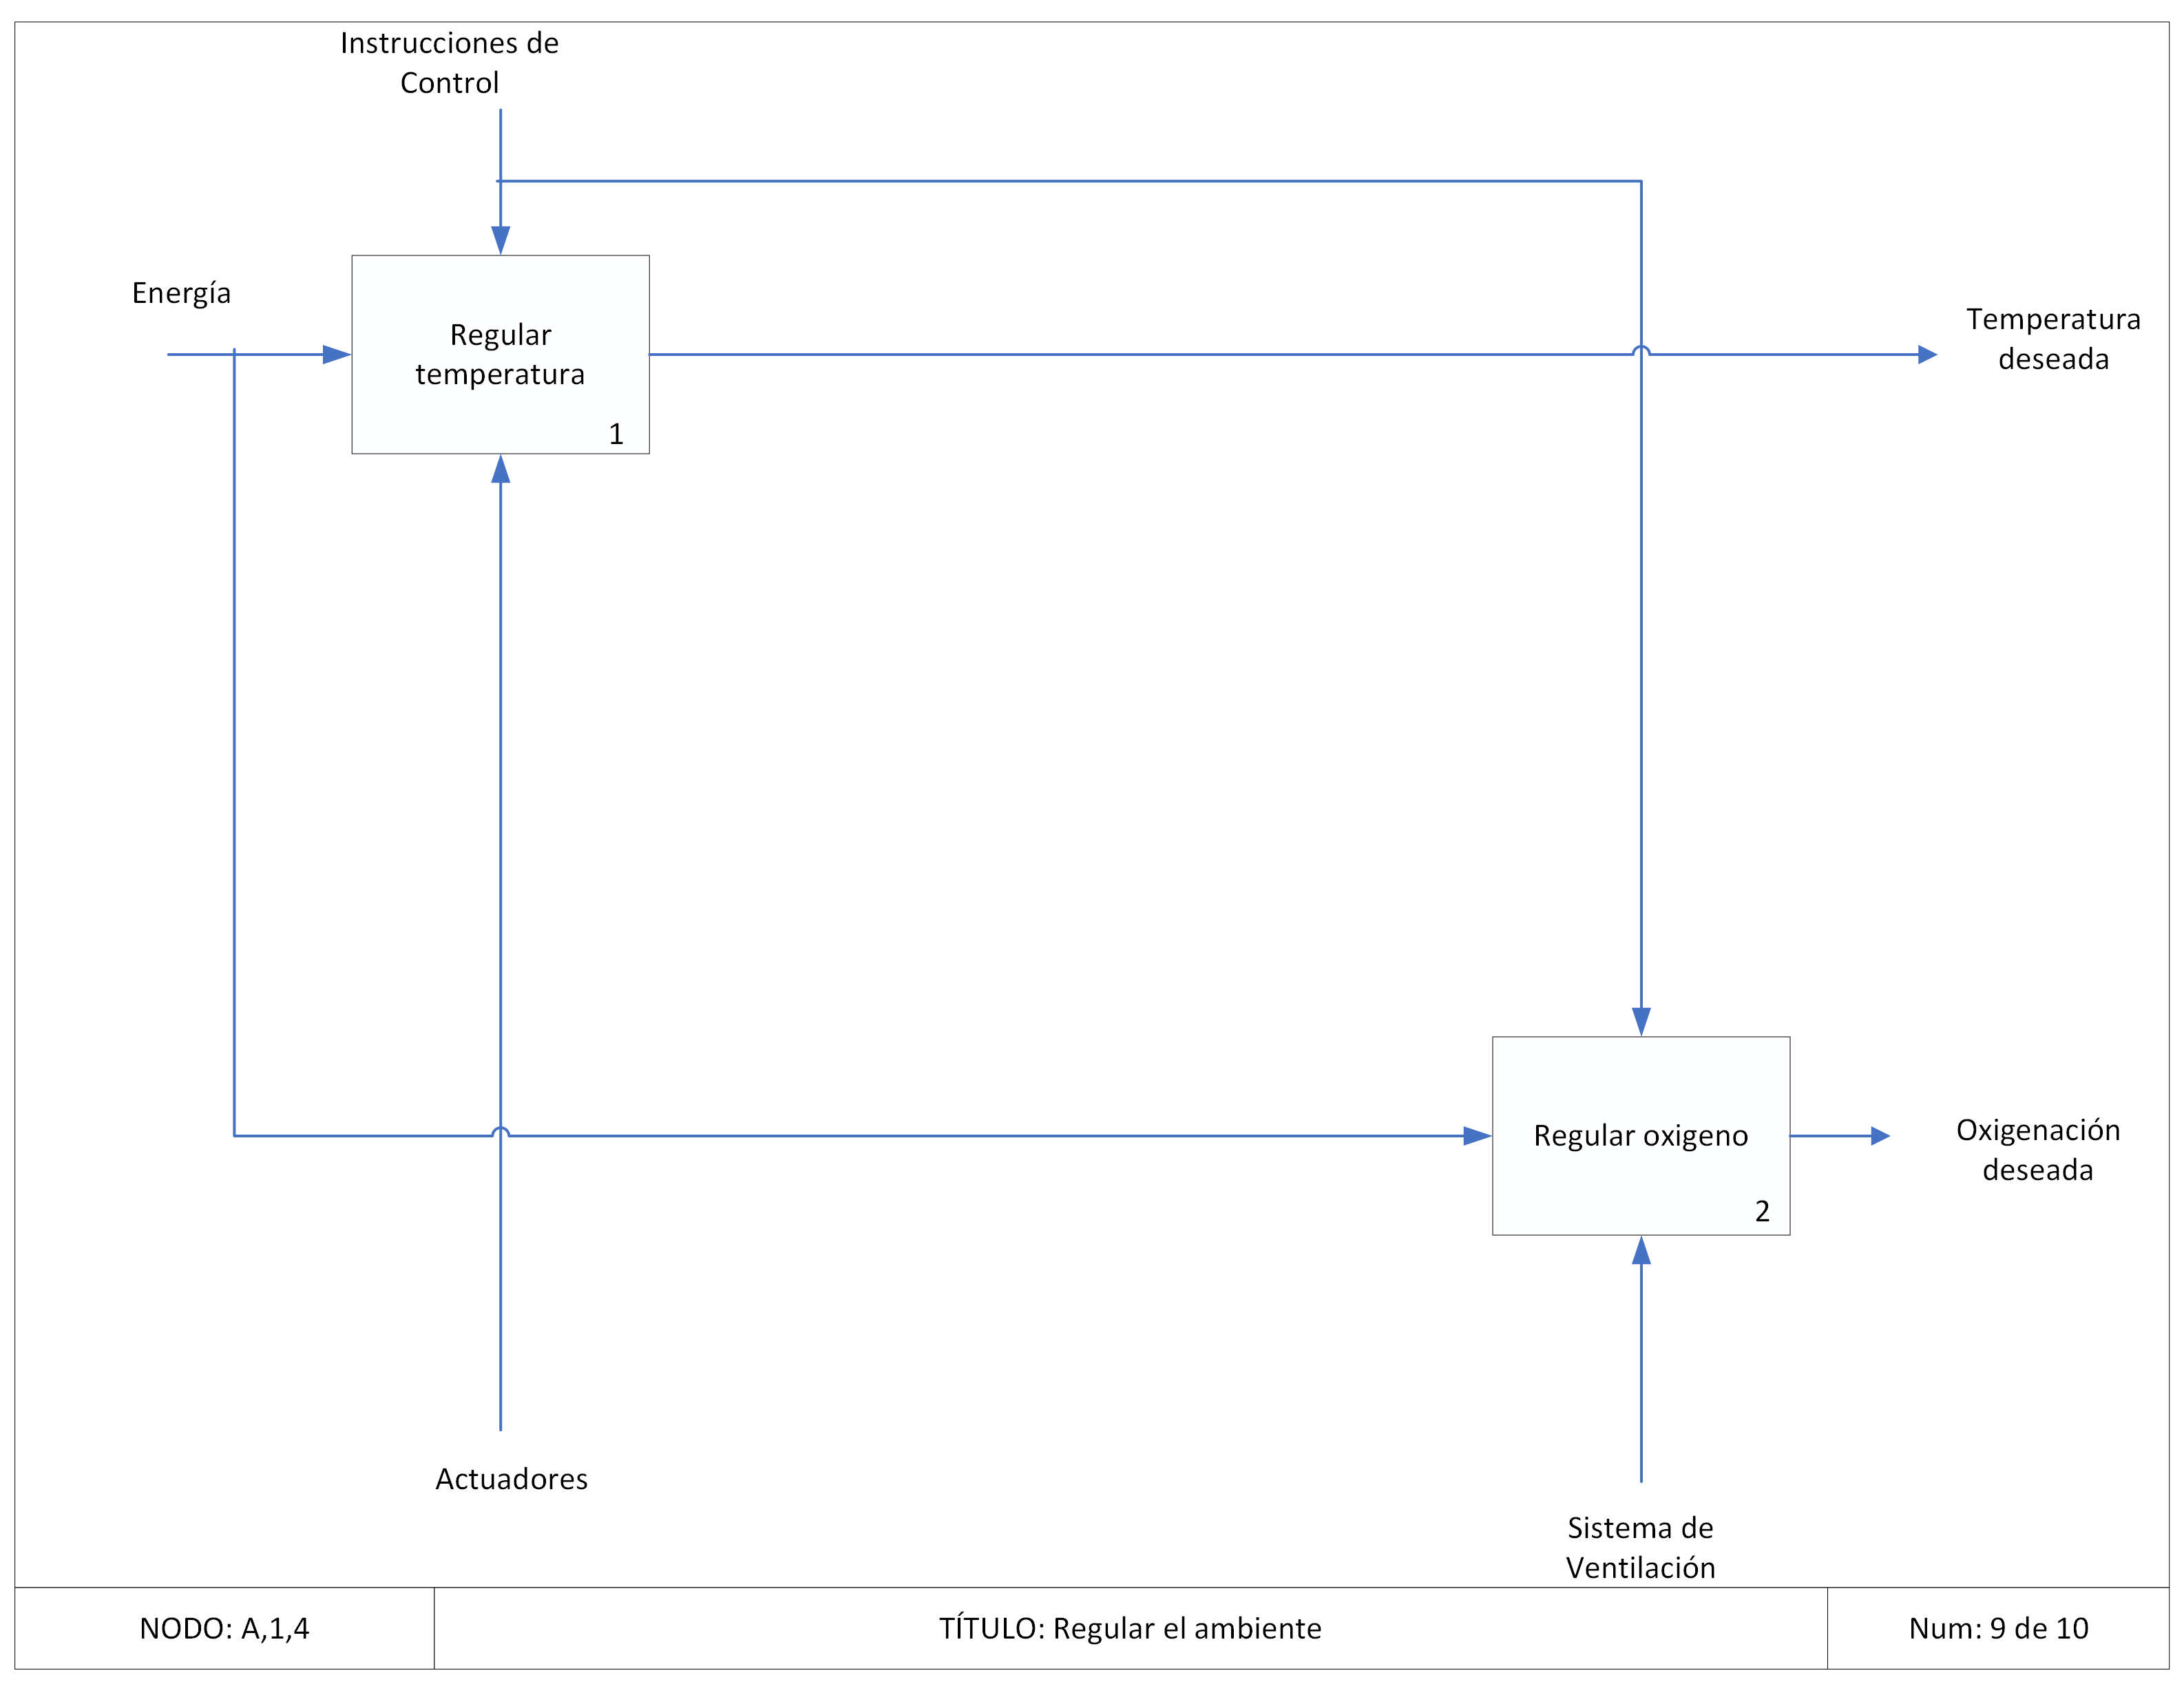
\includegraphics[scale=0.35, angle = 90]{images/Capitulo 6 Apéndices/01 IDEF 0/A,1,4_conmarco - Copy.png}
        \end{figure}
\newpage

\begin{figure}[h]
            \centering
            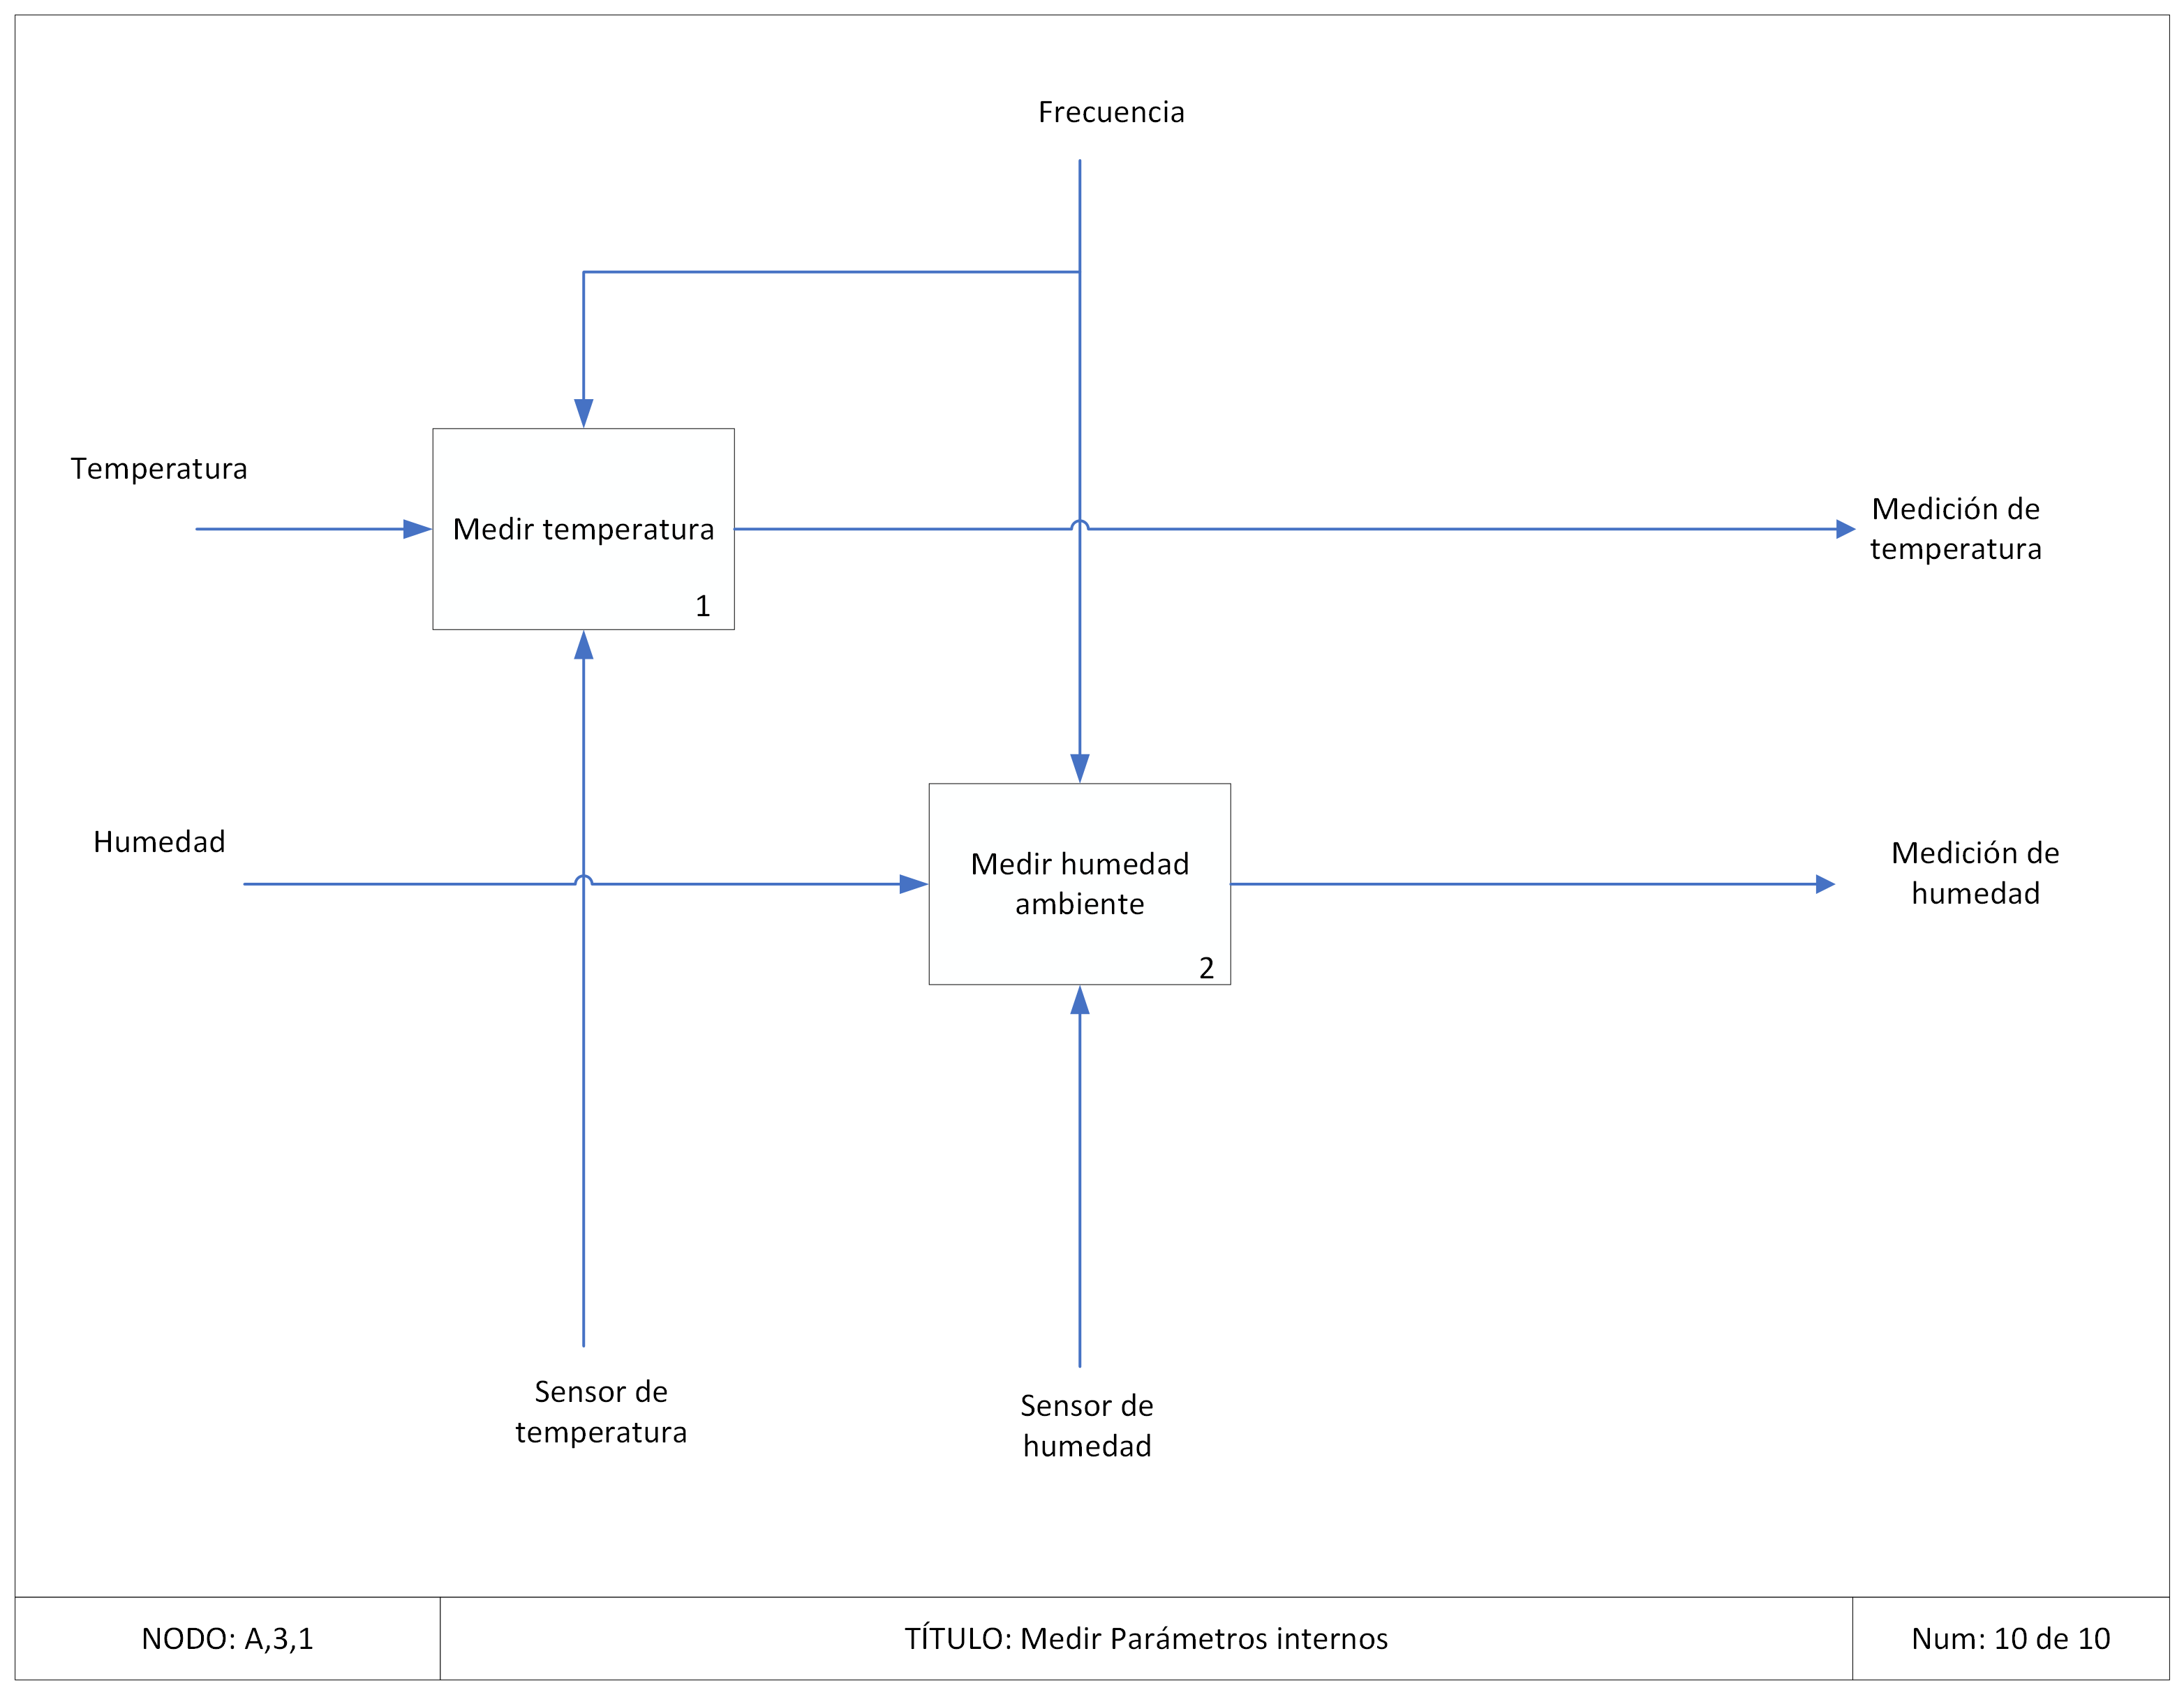
\includegraphics[scale=0.35, angle = 90]{images/Capitulo 6 Apéndices/01 IDEF 0/A,3,1_conmarco - Copy.png}
        \end{figure}
\newpage